\section{Technische Architektur}

\section{Überlegungen zum Technologiestack und der Toolchain}
\label{Technologiestack}

Für die Umsetzung der geplanten Anwendungen gibt es mehre Optionen. Die eingesetzten Technologien, Programmiersprachen und Frameworks bezeichnet man als Technologiestack oder Techstack. Da die Entwicklungsabteilung der IT neu aufgebaut wird, handelt es sich hierbei auch um eine Grundsatzentscheidung, denn obwohl es möglich ist, Folgeprojekte mit einem anderen Techstack durchzuführen hat ein etabliertes und bewährtes Konzept viele Vorteile, vor allem die gewonnen Erfahrung der Mitarbeiter.\\

\subsection{Auswahl der Programmiersprache}

Da viele der Entscheidungen bezüglich der einzusetzenden Anwendungen und Technologien von der verwendeten Programmiersprache Abhängig sind, muss diese Entscheidung getroffen werden, bevor weitere Überlegungen angestellt werden können. Durch den geplanten Anwendungsfall und die Ausbildung der Mitarbeiter der Informationstechnologie Abteilung wurde die Auswahl auf Objektorientierte Programmiersprachen beschränkt, so werden Sprachen, die einem anderen Paradigma folgen wie zum Beispiel funktionale Sprachen nicht in Betracht gezogen.\\

Die Programmiersprache für den Kern der Anwendungen muss einige Anforderungen erfüllen:
\begin{itemize}
  \item Plattformunabhängigkeit (PC, Android und IOS Systeme)
  \item Stabilität und Sicherheit
  \item Zukunftssicherheit
  \item Flexibilität und leichte Zugänglichkeit
\end{itemize}

Aufgrund dieser Anforderungen wurden die neuen Mitarbeiter der Informationstechnologie Abteilung zu einem Workshop eingeladen, der im Vorfeld des eigentlichen Projekts stattfand. Aufgrund der Tragweite der zu treffenden Entscheidung wurde das Format des Lightning Talk gewählt, bei dem jeder Mitarbeiter seine bevorzugte Programmiersprache vorstellen und deren Vorteile herausstellen konnte, moderiert wurde dieser Workshop von Frau Mareike Strauss, die darauf achtete, dass die festgelegte Redezeit nicht überzogen wurde und jeder Teilnehmer gleichberechtigt seine Meinung einbringen konnte.\\ 

Unter den vorgestellten Sprachen befanden sich unter anderem:

\begin{itemize}
  \item Python, C++, Kotlin
  \item Javascript, Java, {C\#}
\end{itemize}

Python hat insbesondere durch die rasante Entwicklung der KI in den letzten Jahren an Bedeutung gewonnen, die Sprache ist relativ leicht zu erlernen und durch eine große Menge an verfügbaren Plugins und Erweiterungen auf viele Anwendungsfälle anpassbar. Allerdings erfüllt Python nicht die gewünschte Zukunftssicherheit, da bereits beim Wechsel von Version 2.7 auf 3.0 Änderungen vorgenommen wurden, die die Abwärtskompatibilität opfern um Optimierungen an der Sprache vorzunehmen. Für den geplanten langfristigen Einsatz einer komplexen Codebasis ist eine solide Kompatibilität über Versionen hinweg jedoch wichtig, da sonst ein notwendiges Update auf eine neue Version langwierige und fehleranfällige Anpassungen nach sich ziehen würde.\\

C++ ist eine gut entwickelte und mächtige Programmiersprache, die vor allem für Hardwarenahe Programmierung eingesetzt wird. Allerdings wird sie (gerade im Vergleich zu moderneren Programmiersprachen als umständlich und kompliziert empfunden. Viele der Teilnehmer schreckte gerade das Konzept der Zeiger und der Header ab, was im Vergleich zu anderen vorgestellten Sprachen von den Workshopteilnehmern als umständlich und kompliziert empfunden wurde. Zudem kann die Speicherverwaltung in C++ gerade für unerfahrene Programmierer schnell zu Fehlern führen, die die gewünschte Stabilität der App gefährden würden.\\

Ein weiterer Vorschlag war es, PhileTipTip als Web-App auf Javascript Basis unter Verwendung von unterschiedlichen Javascript Frameworks (wie React und Next.js) für Front- und Backend umzusetzen. Ein Vorteile bei diesem Vorgehen ist, dass die App unabhängig von Apple und Android auf Mobilgeräte veröffentlich werden kann, da die Nutzer über einen Browser ihrer Wahl auf eine Webseite zugreifen, ohne eine App aus dem Playstore (Android) oder App Store (Apple) herunterladen zu müssen. Gegen diesen Vorschlag spricht der höhere Aufwand, sowohl die Scripte an sich als auch den Server gegen Zugriffe und Manipulation abzusichern, was zwar möglich, aber mangels Erfahrung der Mitarbeiter nicht ohne weiteres umsetzbar wäre.\\

Die Entscheidung fiel nach einer Abstimmung auf Java. Zum einen ist die weite Verbreitung und die Stabilität ein großer Vorteil, es gibt zahlreiche ausgereifte Entwicklungsumgebungen und Plugins für viele Problemstellungen. Durch die große Community ist es sehr wahrscheinlich, schnelle Hilfestellung auf eventuelle Probleme und Antworten auf auftretende Fragen zu erhalten.\\

Ein weiterer Vorteil ist, dass Java gerade im Vergleich zu C++ relativ einsteigerfreundliche, aber dennoch mächtige Programmiersprache ist. Gegenüber Python ist die stärkere Objektorientierung des Sprachkerns ein Vorteil für die Planung und Umsetzung der Systeme, außerdem bietet der LTS (Long Term Support) von Oracle eine Zukunftssicherheit, die bei Versionswechseln von Python nicht unbedingt vorrausgesetzt ist. Gegenüber Kotlin liegen die Vorteile an der weiten Verbreitung und langen Historie der Sprache, die große Community und zahlreichen Frameworks und Plugins. Sollte in der Zukunft die Entscheidung getroffen werden, auf Kotlin umzusteigen wäre dieser Schritt durch die Interoperationalität möglich.\\

Obwohl {C\#} Java in vielen Aspekten stark ähnelt wurde die Entscheidung dennoch für Java getroffen, da nicht geplant wurde, das .Net Ökosystem und verwandte Microsoft Technologien (wie Asp.Net oder Azure) einzusetzen. Durch die starke Ähnlichkeit der Sprachen ist ein Wechsel für zukünftige Projekte, die eine dieser Technologien verwenden sollen mit geringem Aufwand möglich.\\


\subsection{Die Toolchain}

Neben der Programmiersprache und der Datenbanktechnologie gilt es, vor dem Beginn der eigentlichen Entwicklungsarbeit noch einige Entscheidungen bezüglich der einzusetzenden Programme, der Toolchain zu treffen.

\subsubsection{Die IDE}

Die IDE - Integrated Developement Environment (Integrierte Entwicklungsumgebung), diese enthält neben einem Codeeditor mit farblicher Markierung von Schlüsselworten zahlreiche für die Programmierer hilfreiche Funktionalitäten, die sowohl die Entwicklung als auch die Fehlersuche (das Debugging) erleichtern und beschleunigen. So können zum Beispiel Haltepunkte (die sogenannten Breakpoints) gesetzt werden um an bestimmten Stellen die Ausführung des Programms kontrolliert zu unterbrechen und den Programmfluss Schritt für Schritt nachvollziehen zu können.\\

Prinzipiell wäre es natürlich möglich, dass jeder Entwickler eine individuelle Entscheidung bezüglich der Entwicklungsumgebung trifft, aber auch vor dem Hintergrund des Pair Programming ist es sinnvoll, auf eine einheitliche Lösung zurückzugreifen. In diesem Fall soll für die Entwicklung der App Android Studio eingesetzt werden , eine bewährte Java IDE, die mit einer Vielzahl von Plugins angepasst und erweitert werden kann und bereits für die Entwicklung von Android Apps optimiert ist.\\

Für die Entwicklung des Desktop basierten Administrationstools eignet sich Android Studio nur bedingt, daher wird an dieser Stelle auf IntelliJ IDEA zurückgegriffen, welches wie Android Studio von Jetbrains entwickelt wird und somit keine erneute Einarbeitung der Entwickler in eine grundlegend andere IDE (wie zum Beispiel Eclipse) erfordert. Nahezu sämtliche Tastaturkürzel die die Arbeit in Android Studio erleichtern und beschleunigen stehen auch in IntelliJ zur Verfügung und auch die Aufteilung des Arbeitsbereichs ist vertraut und verringert die Transferzeiten und Einarbeitung der Mitarbeiter.\\

\subsubsection{Versionierung}

Ein Versionskontrollsystem erlaubt es mehreren Entwicklern zeitgleich an der selben Codebasis zu entwickeln und Änderungen an den selben Dateien vorzunehmen. Hierfür wird ein zentraler Server verwendet, auf dem der Main-Branch des Projekts liegt, der die Basis für alle verbundenen Entwicklerrechner dient. Hat ein Programmierer eine Teilfunktion abgeschlossen, kann er diese Änderung mit der auf dem Server zusammenführen, wobei Änderungen klar hervorgehoben werden und im Problemfall wieder rückgängig gemacht werden können. Versionskontrollsysteme bieten neben dieser Basisfunktionalität noch weitere hilfreiche Funktionen, wie etwa das Anlegen von mehreren Branches, automatisiertes Builden des Codes und weiteres. Für dieses Projekt wird Git \cite{git}  eingesetzt, eine weit verbreitete Lösung für Versionskontrolle. Um nicht auf die Kommandozeile zurückgreifen zu müssen wird GitGui als grafisches Tool verwendet.\\

Im Gegensatz zu der IDE ist es hier allerdings den Entwicklern freigestellt, ja nach Vorliebe ein alternatives Tool wie zum Beispiel GithubDesktop oder Sourcetree zu verwenden, oder auf Plugins in der IDE zurückzugreifen, da diese Tools lediglich eine einfach bedienbare Oberfläche als Alternative der Kommandozeilenbefehle für die Versionierung zur Verfügung zu stellen. Diese Tools bieten alle einen einfachen Überblick über Änderungen und können auch zur Fehlersuche genutzt werden, indem der fehlerhafte Code mit früheren Versionen verglichen wird.\\

\begin{figure}[!h]
\centering
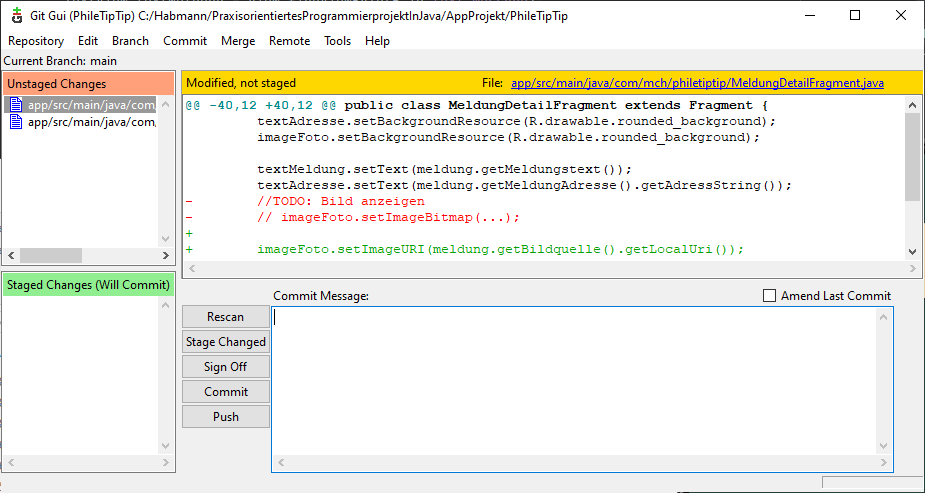
\includegraphics[width=4.63cm, height=2.47cm]{gitgui}
\caption{Git Gui - Grafisches Tool zur Versionsverwaltung}
\end{figure}

Ein weiterer Vorteil, der sich aus der Verwendung eines Versionierungssystems eröffnet ist die Möglichkeit, einen CI/CD Prozess einzubinden. CI steht in diesem Fall für Continous Integration und bedeutet grob gesagt, dass bei jeder Codeänderung die ein Entwickler in das Versionierungssystem hochläd automatische Prozesse losgetreten werden - in der Regel handelt es sich um einen Build Prozess, der diese Änderungen zusammen mit den aktuellen Änderungen der anderen beteiligten Entwickler zusammen zu einer ausführbaren Anwendung zusammensetzt und in der Regel auch vordefinierte Texts durchführen wird, um zu verhindern, dass fehlerhafte und nicht funktionale Codeänderungen in das Endprodukt einfließen.\\

\begin{figure}[!h]
\centering
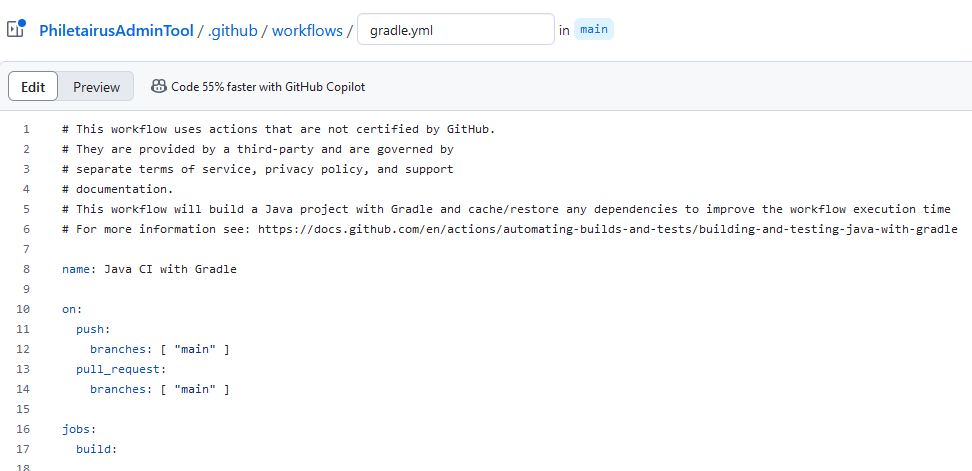
\includegraphics[width=4.86cm, height=2.35cm]{githubactions}
\caption{Github Actions}
\end{figure}

Das CD kann, je nach gewählten Ansatz entweder für Continous Delivery oder Continous Deployment stehen. In beiden Fällen entsteht nach dem CI Schritt ein ausführbares Produkt, was sowohl im Sinne der Scrum Philosophie als auch des Prince2 Prozesses ist. Der Hauptunterschied besteht darin, dass bei Continous Delivery dieses Zwischenprodukt (welches ein Scrum Inkrement darstellen könnte) zunächst manuell freigegeben werden muss, während es bei Continous Deployment sofort nach bestehen der vordefinierten Tests an die angebundenen Nutzer ausgeliefert wird, wodurch diese ständig Zugriff auf die aktuellste Version haben, wodurch die Feedbackschleife deutlich kürzer gestaltet wird, aber unter Umständen auch Zwischenstände von Funktionen, die noch nicht für den Anwendungstest vorgesehen sind veröffentlicht werden können, in beiden Fällen ist eine durchdachte Kommunikationsstrategie notwendig.

%https://www.rapid7.com/de/cybersecurity-grundlagen/cicd/

\subsubsection{Kommunikation und Projektmanagement}

Ein weiteres Tool auf das sich die Projektbeteiligten geeinigt haben ist Jira \cite{jira} - ein Tool über das Tasks verwaltet werden können und das sich in der agilen Softwareentwicklung bewährt hat. Mit Jira können Tickets zu einzelnen Userstories angelegt, bearbeitet und zugeteilt werden, im Sinne der Selbstorganisation natürlich auch von den Entwicklern selbst. Dieses System erleichtert den Überblick für den Product Owner, schafft Übersicht für die Entwickler und auch für den Lenkungsausschuss sowie Projektmanager. Ein weiterer Nebeneffekt ist, dass durch diese digitale Lösung auf Kanban-Boards oder ähnliches verzichtet werden kann wodurch der Nachhaltigkeitsansatz von Prince2 unterstützt wird.\\

%https://support.atlassian.com/jira-software-cloud/docs/what-is-the-connections-feature/
%https://www.techtarget.com/searchsoftwarequality/definition/software-toolchain
%https://www-atlassian-com.translate.goog/devops/devops-tools/choose-devops-tools?_x_tr_sl=en&_x_tr_tl=de&_x_tr_hl=de&_x_tr_pto=rq

\subsubsection{Frameworks und Bibliotheken}

Frameworks sind Sammlungen von Funktionalitäten, die als Paket in das jeweilige Projekt eingebunden werden, um häufig wiederkehrende Probleme und Herausforderungen zu lösen. Häufig vereinfachen Sie Zugriffe auf andere Bibliotheken, indem sie komplizierte Aufrufe vor dem Entwickler verbergen und eine vereinfachte Implementierung gestatten. Eines dieser Frameworks, welches zum Einsatz kommt ist Jitpack, welches eng mit der Versionsverwaltung über Git zusammenarbeitet.\\

\begin{figure}[!h]
\centering
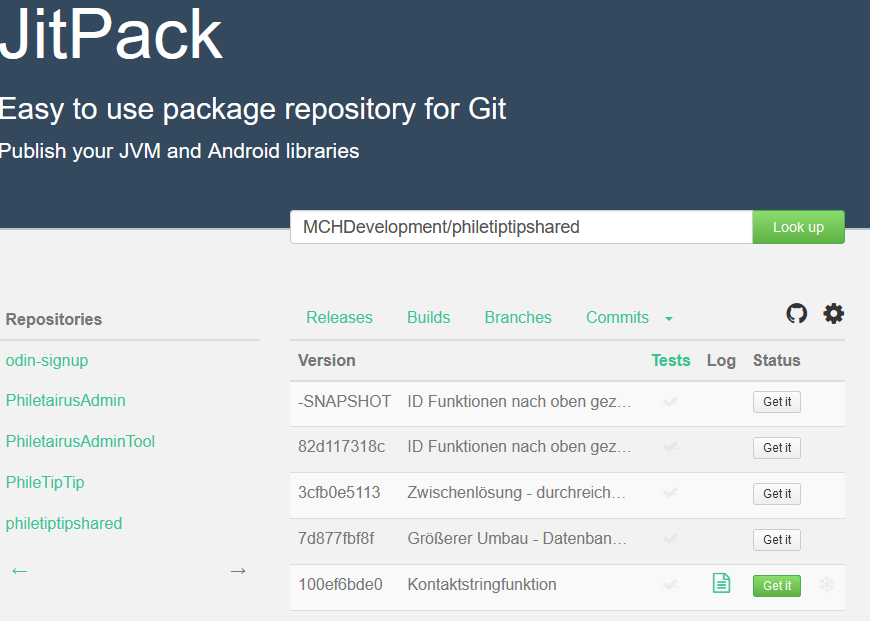
\includegraphics[width=4.35cm, height=3.1cm]{jitpack}
\caption{Jitpack}
\end{figure}

Jitpack erlaubt es, die in einem Repository (Sammlung der hochgeladenen Dateien) befindlichen Klassen und Funktionen in mehreren Projekten einzubinden, ein entscheidender Vorteil für die zweigeteilte Entwicklung PhileTipTip und Phileteirus Admin Tool, die beide auf gemeinsame Datenklassen (etwa für Mieter, Meldungen und Projekte) zugreifen. So müssen Änderungen nur an einer Stelle vorgenommen werden und es kann nicht zu Inkomptibilitäten oder Redundanzen kommen.\\

Neben diesem Framework werden weitere bewährte Lösungen in der Entwicklungen eingesetzt, wie zum Beispiel JavaFX für die Entwicklung der grafischen Oberfläche des Admintools, welches durch die Gestaltung der GUI mithilfe von FXML in Verbindung mit Controller Klassen ein sehr ähnliches Vorgehen wie Android Studio mit der gestaltung über XML Dateien in Verbindung mit Activities ode Fragmenten zur Kontrolle verfolgt.\\ 

FormsFX und ValidatorFX werden für das Erstellen und Verifizieren von Formularen eingesetzt und das bewährte Spring Framework hilft, eine Struktur bereitzustellen, die modernen Ansprüchen gerecht wird und spätere Anbindungen an weitere Dienste und Erweiterungen erleichtert.\\

\subsection{Systemarchitektur}

\subsubsection{Client-Server-Modell}

Sowohl die App PhileTipTip als auch das dazugehörige Philetairus Admin Tool basieren auf einem klassischen Client-Server-Modell, bei dem die App als Client fungiert und über eine API mit einem zentralen Backend kommuniziert. Der Client (die App beziehungsweise die Desktopanwendung) sind für die Datenerfassung durch die Nutzer verantwortlich, während das Backend die Verarbeitung, Speicherung und Verwaltung dieser Daten übernimmt. Dieses Modell ermöglicht eine klare Trennung der Verantwortlichkeiten zwischen der Benutzeroberfläche und der Datenverarbeitung, was zu einer besseren Skalierbarkeit und Flexibilität führt.

\subsubsection{Integration der Datenbank}

Die MySQL-Datenbank ist fest in das Backend integriert und dient als zentrale Speicherinstanz für die erfassten Meldungen, sowie der Datensätze für Mieter, Mitarbeiter, Wohnanlagen und Immobilien. Jede Anfrage des Clients, die eine Datenveränderung oder -abfrage erfordert, wird vom Backend an die Datenbank weitergeleitet. Über definierte API-Endpunkte können Nutzer der App Meldungen zu Schädlingsbefall oder Unkrautbewuchs erstellen und den Status dieser Meldungen abfragen. Gleichzeitig erlaubt das Backend der Grünflächenabteilung, auf diese Daten zuzugreifen, sie zu bearbeiten und den Bearbeitungsstatus zu aktualisieren.\\

Die enge Verzahnung beider Anwendungen ermöglicht es leicht, auf dieser Datenbankstruktur weitere Anwendungen aufzusetzen, um das Vorhaben der vollständigen Digitalisierung des Unternehmens Schritt für Schritt umzusetzen, wobei der Modulare Ansatz und der Modellcharakter dieses Projekts eine solide Basis bilden und die gewonnenen Erfahrungen in weitere Entwicklungen einfließen können.\\

\subsubsection{Backend und API}

Das Backend wird als Vermittler zwischen der App und der Datenbank fungieren. Es nimmt die Anfragen des Clients entgegen, verarbeitet sie und stellt die entsprechenden Daten bereit. Die API, die auf REST-Prinzipien basiert, stellt sicher, dass die Kommunikation zwischen der App und dem Server effizient und sicher erfolgt. Zu den wichtigsten Aufgaben des Backends gehören:

\begin{itemize}
    \item Verarbeitung von Nutzeranfragen: z.B. das Erstellen neuer Meldungen oder das Abrufen bestehender Einträge.
    \item Sicherheit und Authentifizierung: Schutz der Daten durch Zugriffskontrollen und verschlüsselte Kommunikation.
    \item Datenmanagement: Verwaltung und Speicherung der Daten in der MySQL-Datenbank sowie Sicherstellung der Datenintegrität.
\end{itemize}

Diese Architektur sorgt für eine flexible und robuste App, die auf wachsende Nutzerzahlen und Anforderungen skalierbar ist. Zudem ermöglicht sie eine klare Trennung zwischen Frontend (App) und Backend (Datenverarbeitung), was die Wartung und Weiterentwicklung der App erleichtert.

\subsection{Technologien}

\subsubsection{MySQL-Datenbank}

Für die Verwaltung der Anwendungsdaten wird eine MySQL-Datenbank eingesetzt. MySQL ist ein weit verbreitetes relationales Datenbankmanagementsystem, das sich durch seine Zuverlässigkeit, hohe Performance und Skalierbarkeit auszeichnet. Die Datenbank speichert alle wichtigen Informationen, wie Benutzerdaten, Meldungen von Schädlingsbefall oder Unkrautbewuchs und deren Bearbeitungsstatus. Die Anbindung erfolgt über eine API, die die Kommunikation zwischen der App und der Datenbank ermöglicht.

\subsection{Schnittstellen}

\subsubsection{API zur Kommunikation zwischen Frontend und Backend}

Die Kommunikation zwischen dem Frontend (der Android-App) und dem Backend erfolgt über eine RESTful API. Diese API ermöglicht eine klare und strukturierte Interaktion zwischen den beiden Komponenten, indem sie Endpunkte bereitstellt, über die die App auf die vom Backend verwalteten Daten zugreifen kann. Jede Aktion, die von der App ausgeführt wird – sei es das Erfassen einer neuen Meldung von Schädlingsbefall oder das Abrufen des Status einer bestehenden Meldung – erfolgt über HTTP-Anfragen an die API.\\

Die wichtigsten API-Methoden umfassen:
\begin{itemize}
    \item POST: Zum Erstellen neuer Meldungen, die von Nutzern erfasst werden.
    \item GET: Zum Abrufen von Daten, wie z.B. dem Bearbeitungsstatus einer Meldung.
    \item PUT: Zum Aktualisieren von Daten, etwa wenn die Grünflächenabteilung den Status einer Meldung ändert.
    \item DELETE: Für das Löschen von nicht mehr relevanten Daten.
\end{itemize}

Die API ist dabei so konzipiert, dass sie sowohl eine hohe Performance als auch eine sichere Kommunikation gewährleistet. Dies erfolgt durch die Implementierung von HTTPS zur Verschlüsselung der Datenübertragung und einer Token-basierten Authentifizierung, die den Zugriff nur für berechtigte Nutzer und Systeme ermöglicht.

\subsubsection{Benachrichtigungssysteme}

Neben der reinen Datenkommunikation bietet die App ein Benachrichtigungssystem, das die Nutzer über den Status ihrer Meldungen informiert. Diese Benachrichtigungen werden durch das Backend ausgelöst, wenn bestimmte Ereignisse eintreten, wie z.B.:

\begin{itemize}
    \item Eingangsbestätigung einer Meldung: Sobald ein Nutzer eine Meldung abschickt, erhält er eine Bestätigung, dass die Daten erfolgreich erfasst wurden.
    \item Status-Updates: Sobald die Grünflächenabteilung eine Meldung bearbeitet oder den Status ändert, wird der Nutzer per Push-Benachrichtigung informiert.
    \item Erinnerungen: Falls eine Meldung über einen längeren Zeitraum unbeantwortet bleibt, können Erinnerungen an das Bearbeitungsteam oder die Nutzer gesendet werden.
\end{itemize}

Diese Benachrichtigungen werden über Firebase Cloud Messaging (FCM) versendet, das eine zuverlässige und effiziente Zustellung von Push-Benachrichtigungen an die Android-Geräte der Nutzer sicherstellt. So bleiben die Nutzer jederzeit über den Stand ihrer Meldungen informiert, ohne aktiv in der App nachsehen zu müssen.